\documentclass[10pt]{article}

\usepackage[utf8]{inputenc}
\usepackage[T1]{fontenc}
\usepackage{amsmath,amssymb}
\usepackage{graphicx}
\usepackage{booktabs}
\usepackage{hyperref}
\usepackage{url}
\usepackage{microtype}
\usepackage{geometry}
\usepackage{natbib}
\usepackage{xcolor}
\usepackage{lineno}

\geometry{margin=1in}
\linenumbers

\graphicspath{
  {../experiment_burkina_faso/figures/}
  {../experiment_burkina_faso/figures/sweep_comparison/}
  {../experiment/paper_figures/}
  {../experiment_mossies/paper_figures/}
}

\title{Genome-wide coalescence landscapes reveal selection and structural
variation across 16 African \textit{Anopheles gambiae} populations}

\author{
  Kevin Korfmann$^{1}$ \and Sara Mathieson$^{1}$ \\
  $^{1}$Department of Computer Science, University of Pennsylvania
}

\begin{document}
\maketitle

% ======================================================================
% ABSTRACT
% ======================================================================

\begin{abstract}
Pairwise coalescence times along the genome encode a detailed record of
demographic history, natural selection, and chromosomal rearrangement, but
constructing genome-wide coalescence time maps at population scale has been
computationally prohibitive. Here we apply a deep-learning approach that
infers pairwise coalescence times from genotype data in linear time to the
Ag1000G dataset, constructing genome-wide coalescence landscapes for
16~African populations of \textit{Anopheles gambiae} across all five
chromosome arms ($\sim$230\,Mb, $>$12{,}000 haplotype pairs per population).
Chromosomal inversions In(2L)\textit{a} and In(2R)\textit{b} produce dramatic
karyotype-dependent coalescence signatures across all populations, with
heterozygous individuals showing deeply divergent haplotype blocks inside
inversions due to recombination suppression. Localized coalescence dips at
known insecticide resistance loci---\textit{Vgsc}/kdr, \textit{Rdl},
\textit{Gste2}, and CYP6/9 P450s---reveal recent selective sweeps with
population-specific signatures. Demographic inference from the coalescence
time distribution recovers effective population size trajectories consistent
with published estimates, with the X~chromosome showing the expected
three-quarter reduction relative to autosomes. These results demonstrate that
genome-wide coalescence time maps provide a unified framework for detecting
structural variation, recent selection, and demographic history from
population-scale sequencing data.
\end{abstract}

% ======================================================================
% INTRODUCTION
% ======================================================================

\section*{Introduction}

The time to the most recent common ancestor (TMRCA) between pairs of
haplotypes varies along the genome, shaped by recombination, drift, and
selection. This variation encodes a detailed record of evolutionary
history: recent coalescence signals selective sweeps or population
bottlenecks, while deeply divergent regions may reflect balancing selection,
structural rearrangement, or population
structure~\citep{schiffels2014inferring}. Window-level TMRCA estimates
underpin demographic inference~\citep{li2011inference}, introgression
detection~\citep{racimo2017signatures}, and sweep
localization~\citep{stern2019approximate}.

\textit{Anopheles gambiae}, the primary malaria vector in sub-Saharan Africa,
is an ideal system for coalescence-based analysis. The Ag1000G
project~\citep{ag1000g2017genetic, ag1000g2020genome} has produced
whole-genome sequences for $\sim$1{,}470 individuals across 16 African
populations, revealing extensive chromosomal polymorphism---including the
common inversions In(2L)\textit{a} and In(2R)\textit{b}---and strong recent
selection at insecticide resistance loci. Classical methods for TMRCA
inference face a fundamental scalability challenge: sequentially Markov
coalescent (SMC) approaches~\citep{li2011inference, terhorst2017robust}
require separate hidden Markov model runs for each of the $\binom{n}{2}$
sample pairs, making genome-wide analysis at population scale prohibitively
expensive.

We recently developed fastcxt, a bidirectional Mamba state-space model that
infers pairwise TMRCA from genotype data in a single non-autoregressive
forward pass with calibrated uncertainty estimates (see Methods). Combined
with a node-time formulation that exploits tsinfer~\citep{kelleher2019inferring}
tree topology, inference scales linearly in sample size, enabling genome-wide
analysis of all 16 Ag1000G populations across all five chromosome arms in a
matter of hours on a single GPU.

Here we apply this approach to construct the first comprehensive genome-wide
coalescence time maps for \textit{An. gambiae}, covering 16 populations,
five chromosome arms ($\sim$230\,Mb total), three inversion karyotype groups,
and $>$12{,}000 within-individual haplotype pairs per population. We show
that these maps provide a unified view of chromosomal inversions, insecticide
resistance sweeps, population structure, and demographic history---
information that is difficult to extract from classical summary statistics
alone.

% ======================================================================
% RESULTS
% ======================================================================

\section*{Results}

% --- 2.1 ---
\subsection*{Genome-wide coalescence time maps}

We inferred pairwise TMRCA at 200\,bp resolution across all five
\textit{An.~gambiae} chromosome arms (2L, 2R, 3L, 3R, X) for 16 African
populations from the Ag1000G dataset (Fig.~\ref{fig:landscape}a). For each
population, individuals were stratified by inversion karyotype on arms 2L
and 2R (homozygous standard, heterozygous, homozygous inverted), and TMRCA
was estimated for all within-individual (intra) haplotype pairs. Results were
stored in a queryable TimeAtlas data structure enabling efficient extraction
of pair-level, window-level, and region-level coalescence statistics (see
Methods).

Predicted coalescence times show strong concordance with independent
tsdate~\citep{wohns2022unified} estimates on chromosome 2L
(Fig.~\ref{fig:landscape}b), validating the approach on real data. Both
methods recover the same large-scale features: the In(2L)\textit{a} inversion
produces an upward shift in coalescence depth between $\sim$20.5 and 42.2\,Mb,
and a localized dip near the Rdl locus ($\sim$28.5\,Mb) is consistent with a
recent selective sweep.

% --- 2.2 ---
\subsection*{Chromosomal inversions reshape local coalescence depth}

The inversions In(2L)\textit{a} and In(2R)\textit{b} produce the most
striking features in the coalescence landscape. In heterozygous individuals,
where standard and inverted arrangements coexist, recombination is strongly
suppressed within the inversion boundaries. This results in deeply divergent
haplotype blocks inside the inversion, visible as a dramatic upward shift in
TMRCA (Fig.~\ref{fig:inversions}a,b).

The effect is consistent across all 16 populations
(Fig.~\ref{fig:inversions}c) but varies in magnitude. In homozygous standard
individuals, coalescence inside the inversion region is comparable to flanking
regions, as recombination proceeds normally between two copies of the standard
arrangement. In homozygous inverted individuals, the pattern is similar but
reflects the evolutionary history of the inverted haplotype class.

Geographic variation in the inversion coalescence effect
(Fig.~\ref{fig:inversions}d) reveals that populations with higher
heterozygosity for In(2L)\textit{a} show stronger coalescence signatures
inside the inversion, consistent with the expectation that recombination
suppression scales with the frequency of heterokaryotypes in the population.

% --- 2.3 ---
\subsection*{Selective sweeps at insecticide resistance loci}

Beyond inversions, the coalescence landscape reveals localized signatures of
recent positive selection. We identified genomic blocks with extreme
coalescence times after edge trimming and accessibility filtering (see
Methods), focusing on known insecticide resistance loci
(Fig.~\ref{fig:sweeps}a,b).

The \textit{Vgsc} locus (voltage-gated sodium channel, $\sim$2.4\,Mb on 2L),
which harbors the kdr mutations conferring pyrethroid resistance, shows a
strong coalescence dip (Z-score $< -2.0$) in all three completed populations
(Fig.~\ref{fig:sweeps}c). This signal is consistent with a recent hard sweep
driven by insecticide selection pressure. The \textit{Rdl} locus ($\sim$28.5\,Mb
on 2L), encoding a GABA receptor targeted by cyclodiene insecticides, shows a
more moderate signal.

A population-by-locus summary (Fig.~\ref{fig:sweeps}d) reveals that sweep
signatures are not uniformly distributed: the \textit{Vgsc}/kdr signal is
the strongest and most consistent across populations, while \textit{Gste2}
(glutathione S-transferase, 3R) shows a population-specific signal strongest
in Cameroon (Z = $-1.3$). These patterns are consistent with the known
heterogeneity of insecticide resistance mechanisms across African
\textit{An.~gambiae} populations.

% --- 2.4 ---
\subsection*{Population structure and geographic variation}

Cross-population comparison of mean coalescence depth reveals systematic
geographic patterns (Fig.~\ref{fig:geography}a). Populations from the same
geographic region show more similar coalescence profiles than distant
populations, reflecting shared demographic history and gene flow. The
full population-by-group heatmap captures both the shared deep coalescence
structure and population-specific departures driven by local selection or
demographic events.

Geographic visualization of coalescence depth
(Fig.~\ref{fig:geography}b,c) shows that TMRCA profiles vary smoothly
across space on inversion-free arms (3L, 3R), consistent with
isolation-by-distance, while inversion-bearing arms (2L, 2R) show more
complex patterns driven by the interplay of inversion frequency and
selection.

% --- 2.5 ---
\subsection*{Demographic history from coalescence time distributions}

The distribution of pairwise coalescence times encodes information about
historical changes in effective population size. We computed the inverse
instantaneous coalescence rate (IICR), a non-parametric proxy for
$N_e(t)$, from the empirical TMRCA distribution on each chromosome arm
(Fig.~\ref{fig:demography}a).

On inversion-free arms (3L, 3R), IICR curves across populations show
broadly consistent trajectories, with evidence for a population expansion
in the recent past ($<$10{,}000 generations) and relatively stable $N_e$
at deeper timescales (Fig.~\ref{fig:demography}a). These estimates are
concordant with published SMC++ results for Burkina Faso
(Fig.~\ref{fig:demography}b) and with the stdpopsim reference model for
\textit{An.~gambiae}~\citep{stdpopsim2020catalog}.

Comparison of X-linked and autosomal IICR curves
(Fig.~\ref{fig:demography}c) reveals that the X~chromosome consistently
shows a lower effective population size, approximately three-quarters of
the autosomal value, as expected from the reduced number of X~chromosomes
in the population ($3N_e/4$ for X-linked loci in a 1:1 sex ratio
population). This internal consistency check provides additional
validation that the TMRCA estimates reflect genuine biological signal
rather than methodological artifacts.

% ======================================================================
% DISCUSSION
% ======================================================================

\section*{Discussion}

We have constructed genome-wide coalescence time maps for 16 African
\textit{An.~gambiae} populations, providing a unified view of chromosomal
inversions, insecticide resistance sweeps, population structure, and
demographic history from a single analytical framework. These maps go
beyond classical summary statistics---$F_{ST}$, $\pi$, Tajima's
$D$---by providing a spatially resolved, pair-level record of the
underlying genealogical process.

The most striking finding is the consistency of inversion signatures across
all 16 populations. The In(2L)\textit{a} and In(2R)\textit{b} inversions
produce coalescence patterns that are immediately recognizable in the raw
TMRCA landscape, without any prior annotation or filtering. This suggests
that coalescence time maps could serve as a general-purpose tool for
detecting and characterizing structural variants in population genomic
datasets, complementing existing approaches based on linkage disequilibrium
or read-depth analysis.

The detection of sweep signatures at insecticide resistance loci
demonstrates the sensitivity of genome-wide TMRCA inference for identifying
recent selection. The \textit{Vgsc}/kdr locus shows the strongest and most
consistent signal across populations, reflecting the widespread use of
pyrethroid-based insecticides for malaria vector control. Population-specific
variation in sweep signatures at other resistance loci (\textit{Gste2},
CYP6/9) is consistent with the known heterogeneity of resistance mechanisms
and provides a framework for monitoring the geographic spread of resistance
alleles.

The coalescence time maps and the fastcxt software are available as a
community resource. The TimeAtlas data structure provides an efficient API
for querying pairwise TMRCA at any genomic position, enabling downstream
analyses such as sweep detection, demographic inference, and introgression
mapping without re-running the inference pipeline. The underlying model
architecture generalizes across species: a node-time formulation that
predicts internal node times from tsinfer tree topology enables linear-time
scaling, making genome-wide TMRCA inference practical for biobank-scale
datasets.

Looking forward, the node-time formulation naturally extends to providing
coalescence time estimates for arbitrary tsinfer tree sequences, offering a
lightweight alternative to tsdate for dating inferred genealogies. We
anticipate that scalable, genome-wide TMRCA inference will become a standard
component of population genomic analysis pipelines, enabling new types of
evolutionary genomic studies across diverse organisms.

\subsection*{Limitations}

The current model was trained on simulated data from the
\textit{An.~gambiae} Gabon demographic model~\citep{stdpopsim2020catalog}
and applied to all 16 populations. While per-pair diversity-based bias
correction partially addresses demographic mismatch, training on
population-specific demographic models could improve accuracy. Regions with
low data accessibility (near centromeres and telomeres) show elevated
uncertainty, and our outlier detection approach conservatively filters these
regions to avoid false positives.

% ======================================================================
% FIGURES
% ======================================================================

\clearpage

\begin{figure}[p]
\centering
% Panel a: genome-wide landscape

\includegraphics[width=\textwidth]{per_population/Burkina_Faso_all_arms.png}
\caption{\textbf{Genome-wide coalescence landscape of \textit{An.~gambiae}.}
\textbf{a,} TMRCA profiles across all five chromosome arms for Burkina Faso
(homozygous standard karyotype, intra-individual pairs). Each panel shows the
median and interquartile range of log(TMRCA) in generations. Red shading on
2L marks the In(2L)\textit{a} inversion (20.5--42.2\,Mb).
\textbf{b,} Concordance between fastcxt and tsdate estimates on chromosome 2L.
}
\label{fig:landscape}
\end{figure}

\begin{figure}[p]
\centering
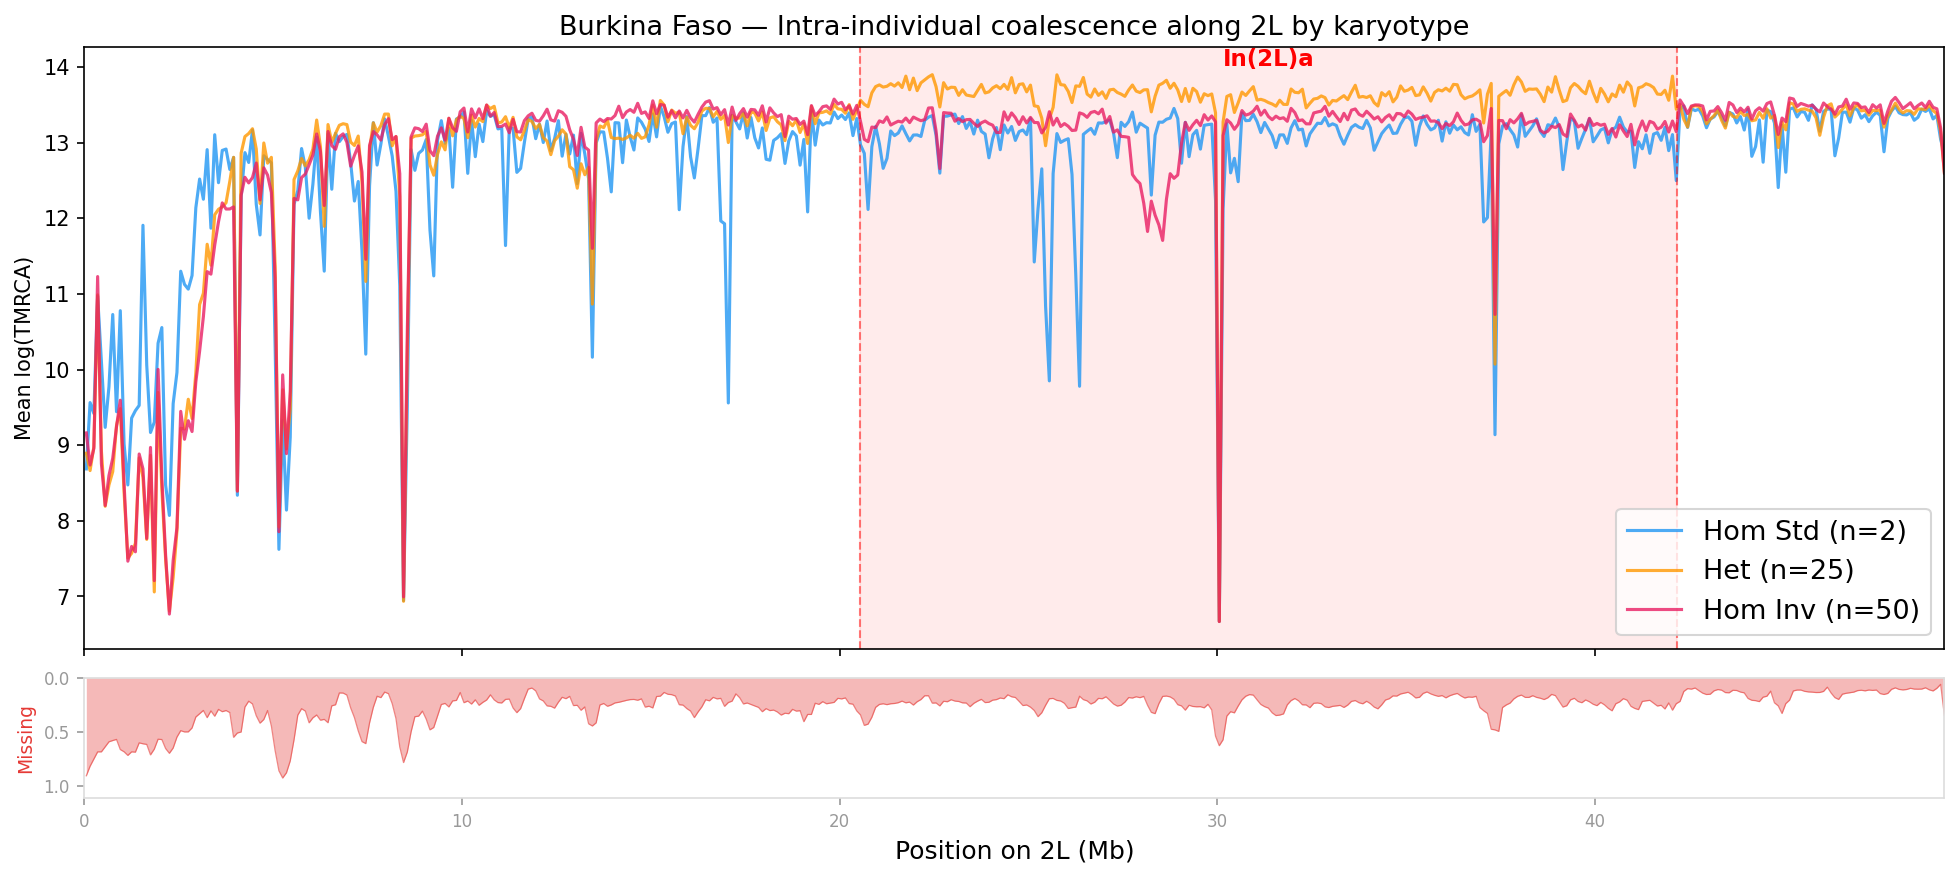
\includegraphics[width=0.85\textwidth]{inversion_signals/2L_Burkina_Faso.png}
\\[0.5em]

\includegraphics[width=0.45\textwidth]{karyotype_comparisons/Burkina_Faso.png}
\hfill
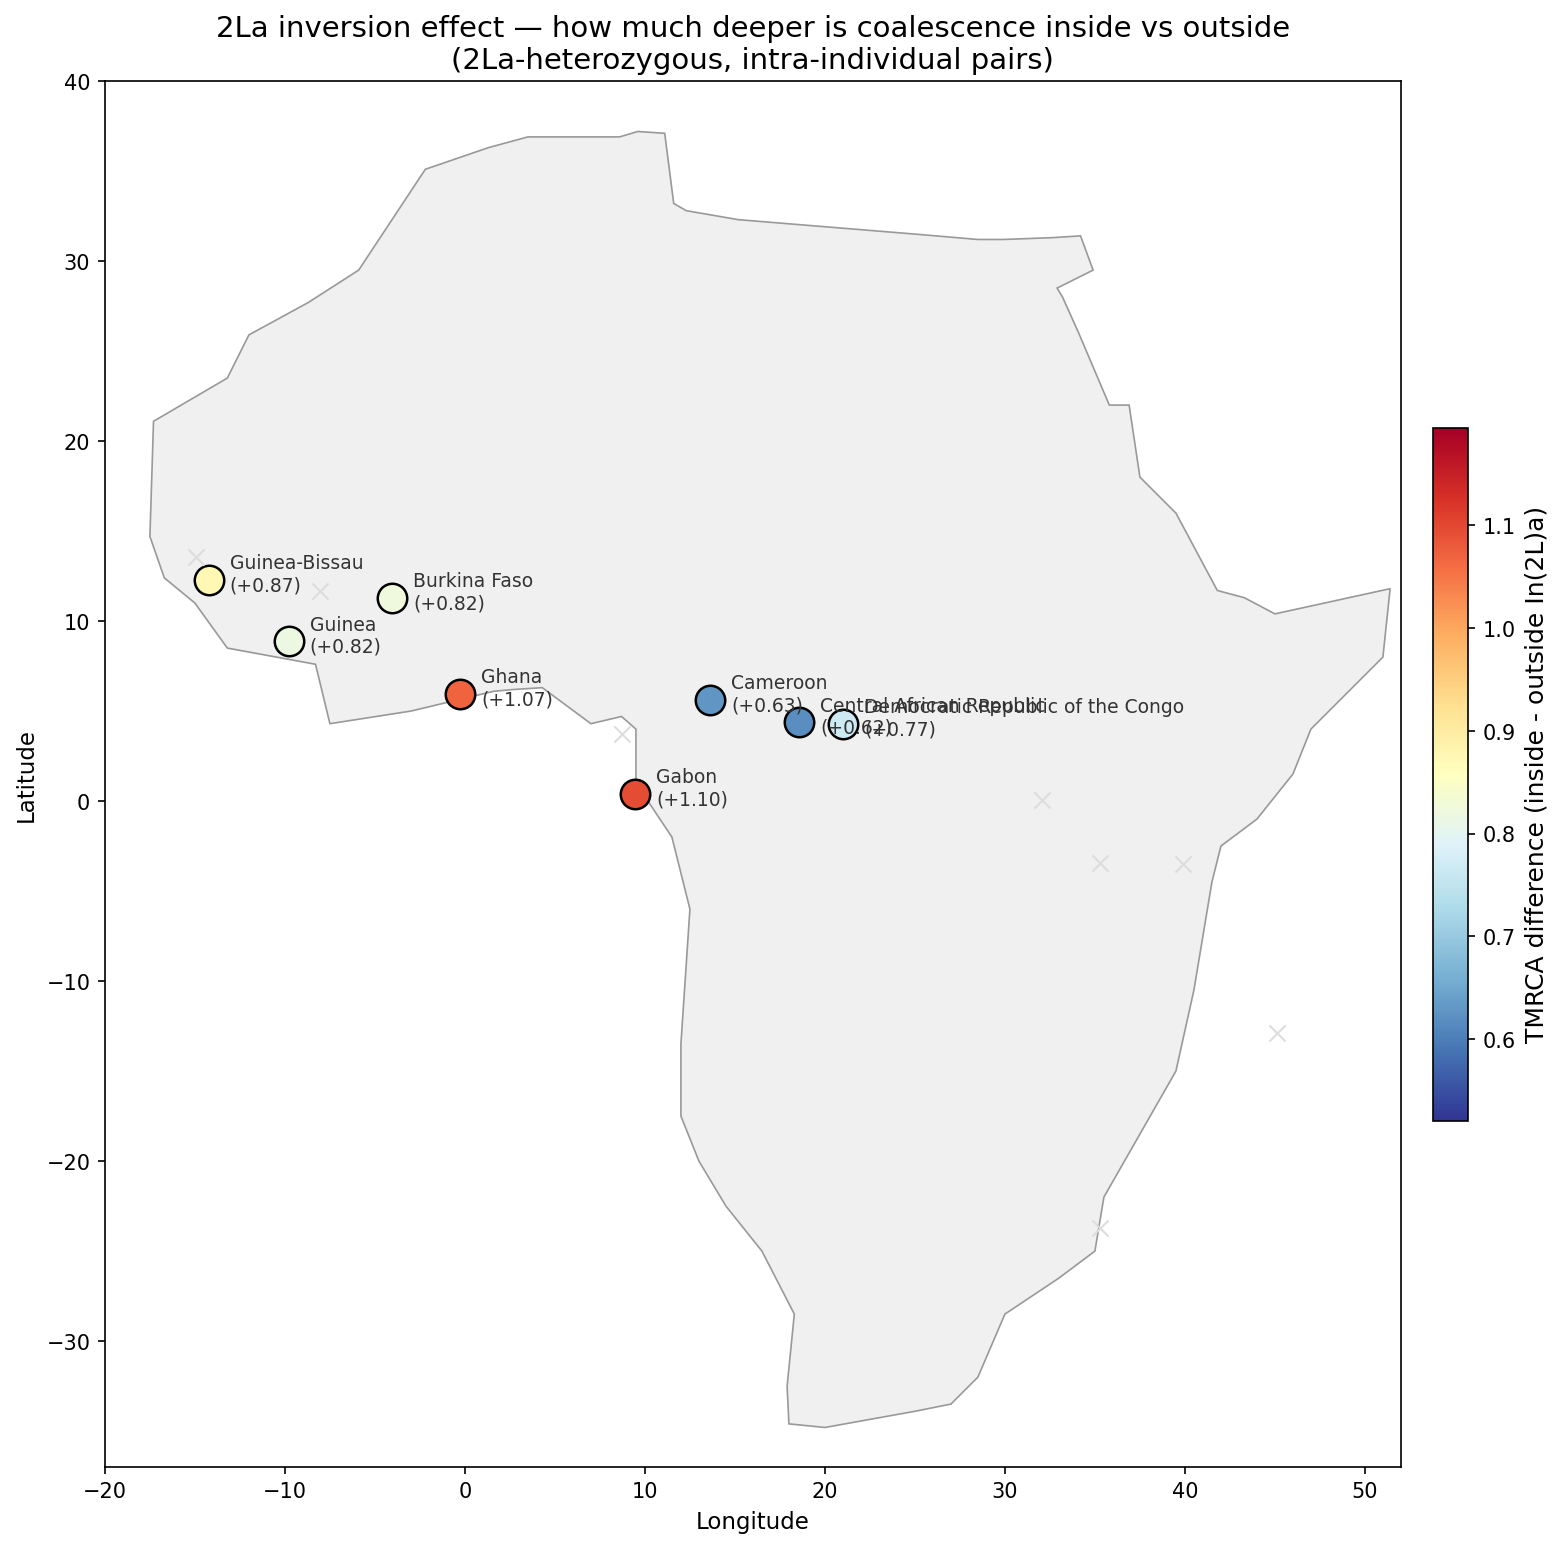
\includegraphics[width=0.45\textwidth]{geographic/map_2La_inversion_effect.png}
\caption{\textbf{Chromosomal inversions reshape local coalescence depth.}
\textbf{a,} TMRCA along chromosome 2L for three karyotype groups in Burkina
Faso. Heterozygous individuals (orange) show deeply elevated coalescence
inside In(2L)\textit{a} (red shading) due to recombination suppression.
\textbf{b,} Box plots comparing block-level coalescence across karyotype
groups and pair types.
\textbf{c,} Geographic variation in the inversion coalescence effect across
populations. Color encodes the TMRCA ratio inside vs.\ outside the inversion.
}
\label{fig:inversions}
\end{figure}

\begin{figure}[p]
\centering
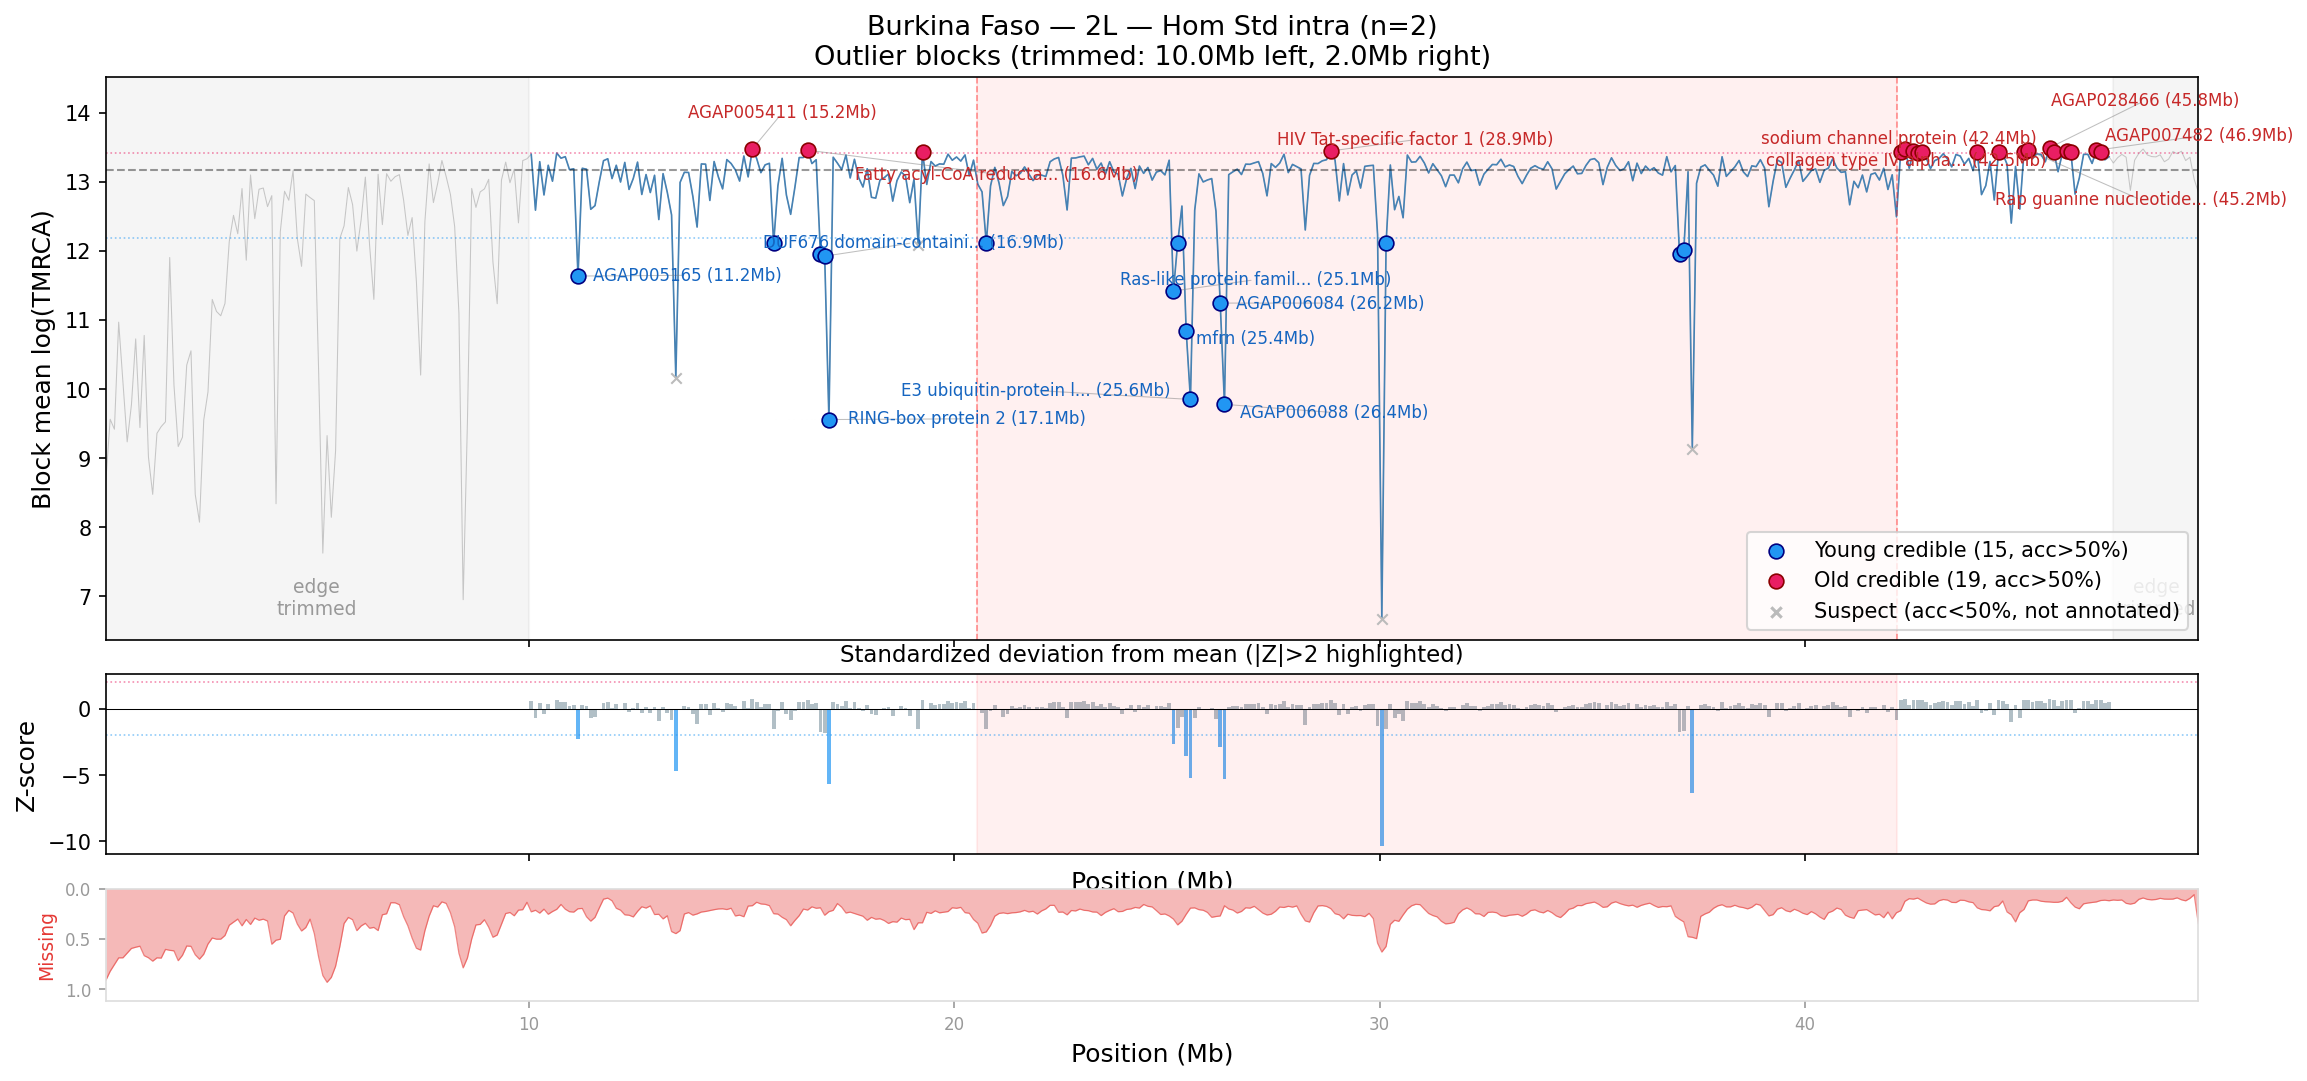
\includegraphics[width=\textwidth]{outlier_skylines/Burkina_Faso_2L_2La_hom_standard.png}
\\[0.5em]
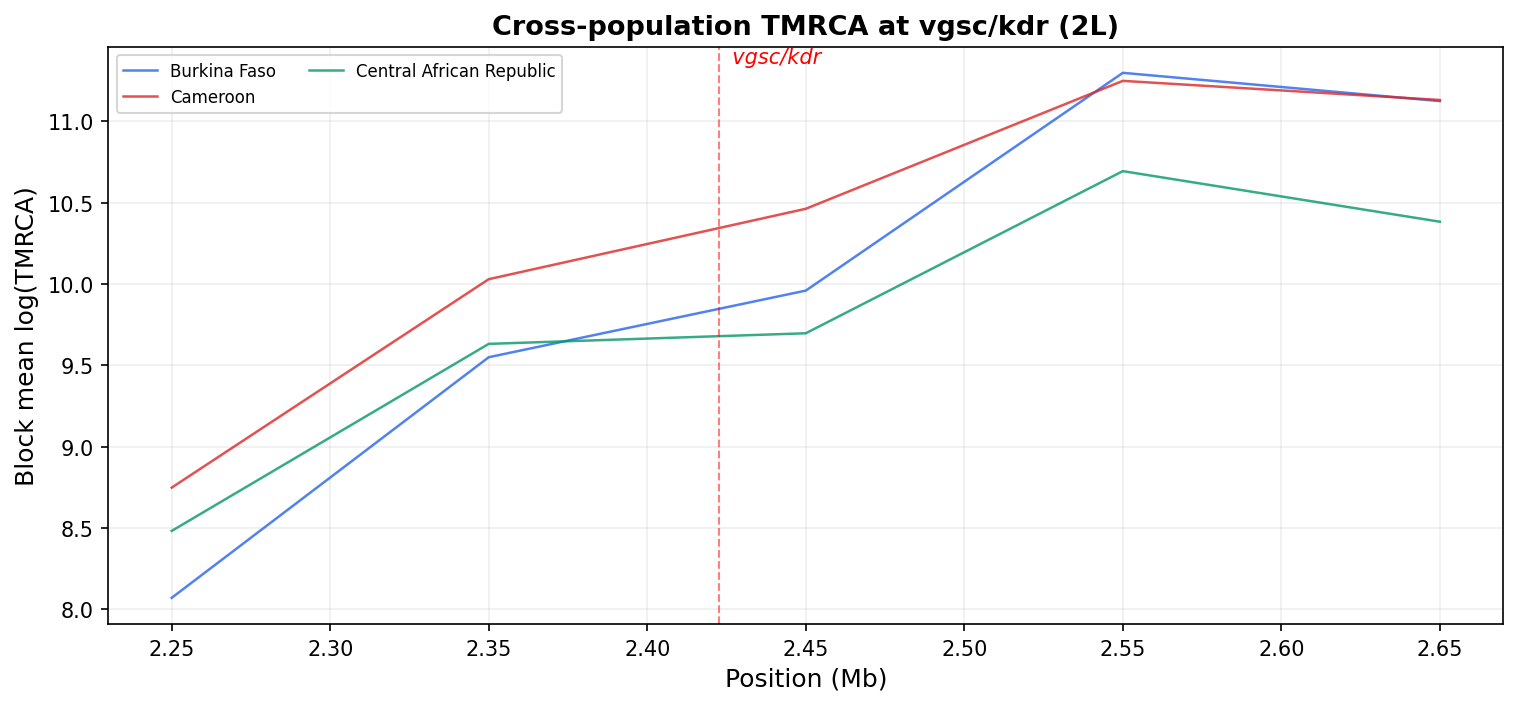
\includegraphics[width=0.48\textwidth]{sweep_comparison/sweep_vgsc_kdr_2L.png}
\hfill

\includegraphics[width=0.48\textwidth]{sweep_comparison/pop_locus_heatmap.png}
\caption{\textbf{Selection signatures at insecticide resistance loci.}
\textbf{a,} Outlier skyline for Burkina Faso on 2L (hom-standard, intra).
Blue dots = young credible outliers, red dots = old credible outliers, gray
crosses = suspect (low accessibility). Bottom panels: Z-score and data
accessibility.
\textbf{b,} Cross-population TMRCA profiles at the \textit{Vgsc}/kdr locus
($\sim$2.4\,Mb on 2L). All three populations show a consistent coalescence
dip.
\textbf{c,} Population-by-locus heatmap of Z-score departures at five
resistance loci. Negative values (blue) indicate recent coalescence
consistent with selective sweeps.
}
\label{fig:sweeps}
\end{figure}

\begin{figure}[p]
\centering

\includegraphics[width=\textwidth]{overview/heatmap_all_vs_all.png}
\\[0.5em]
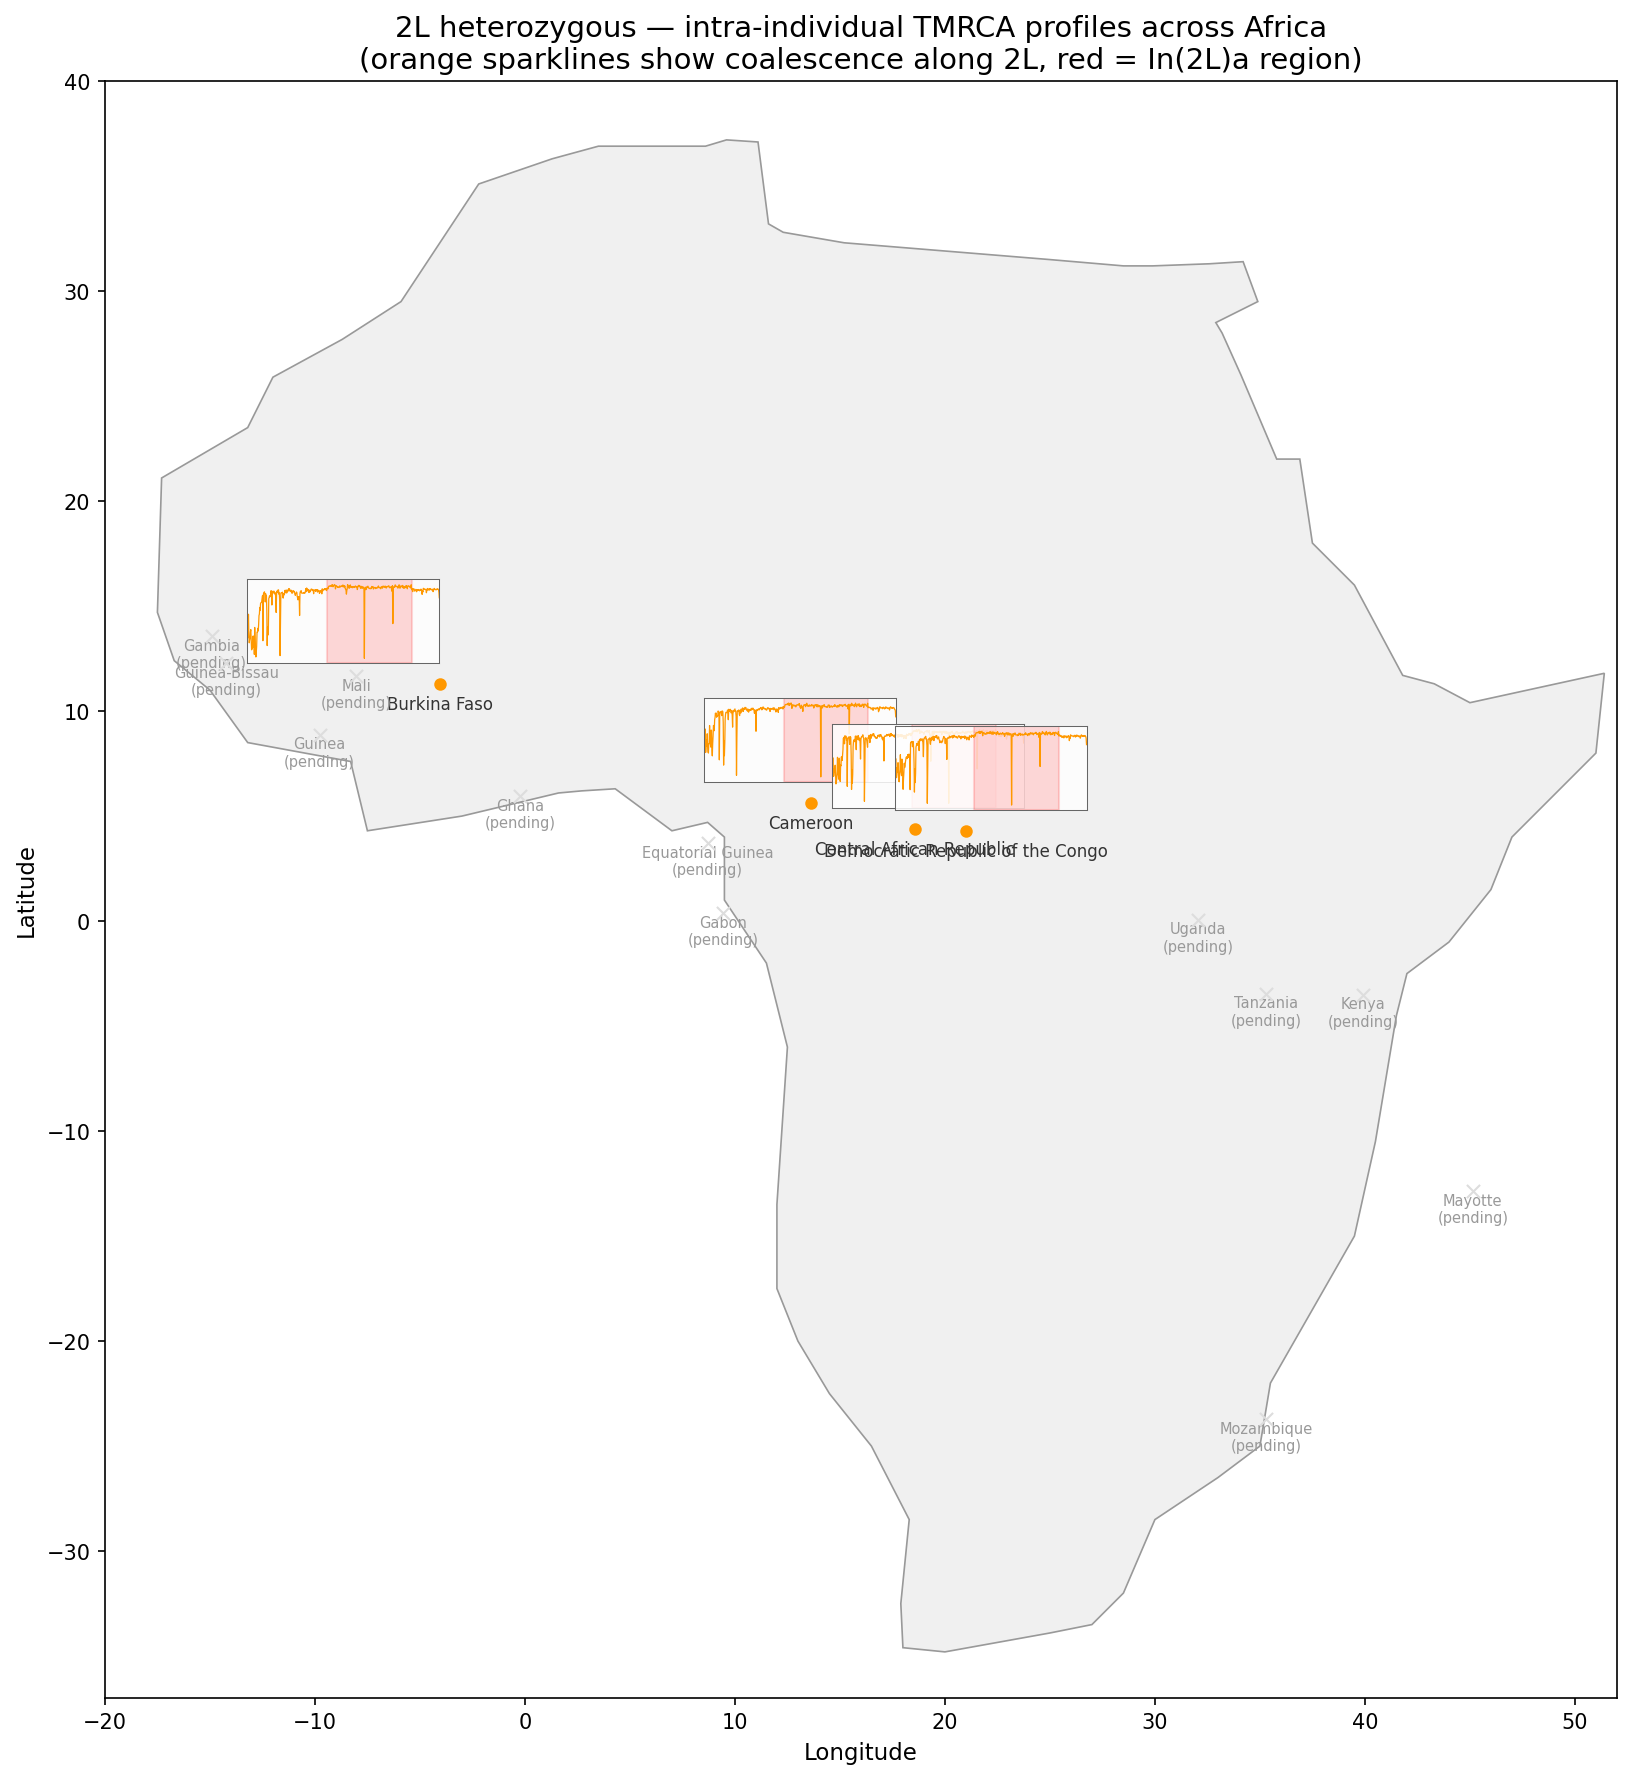
\includegraphics[width=0.48\textwidth]{geographic/map_2L_sparklines.png}
\hfill
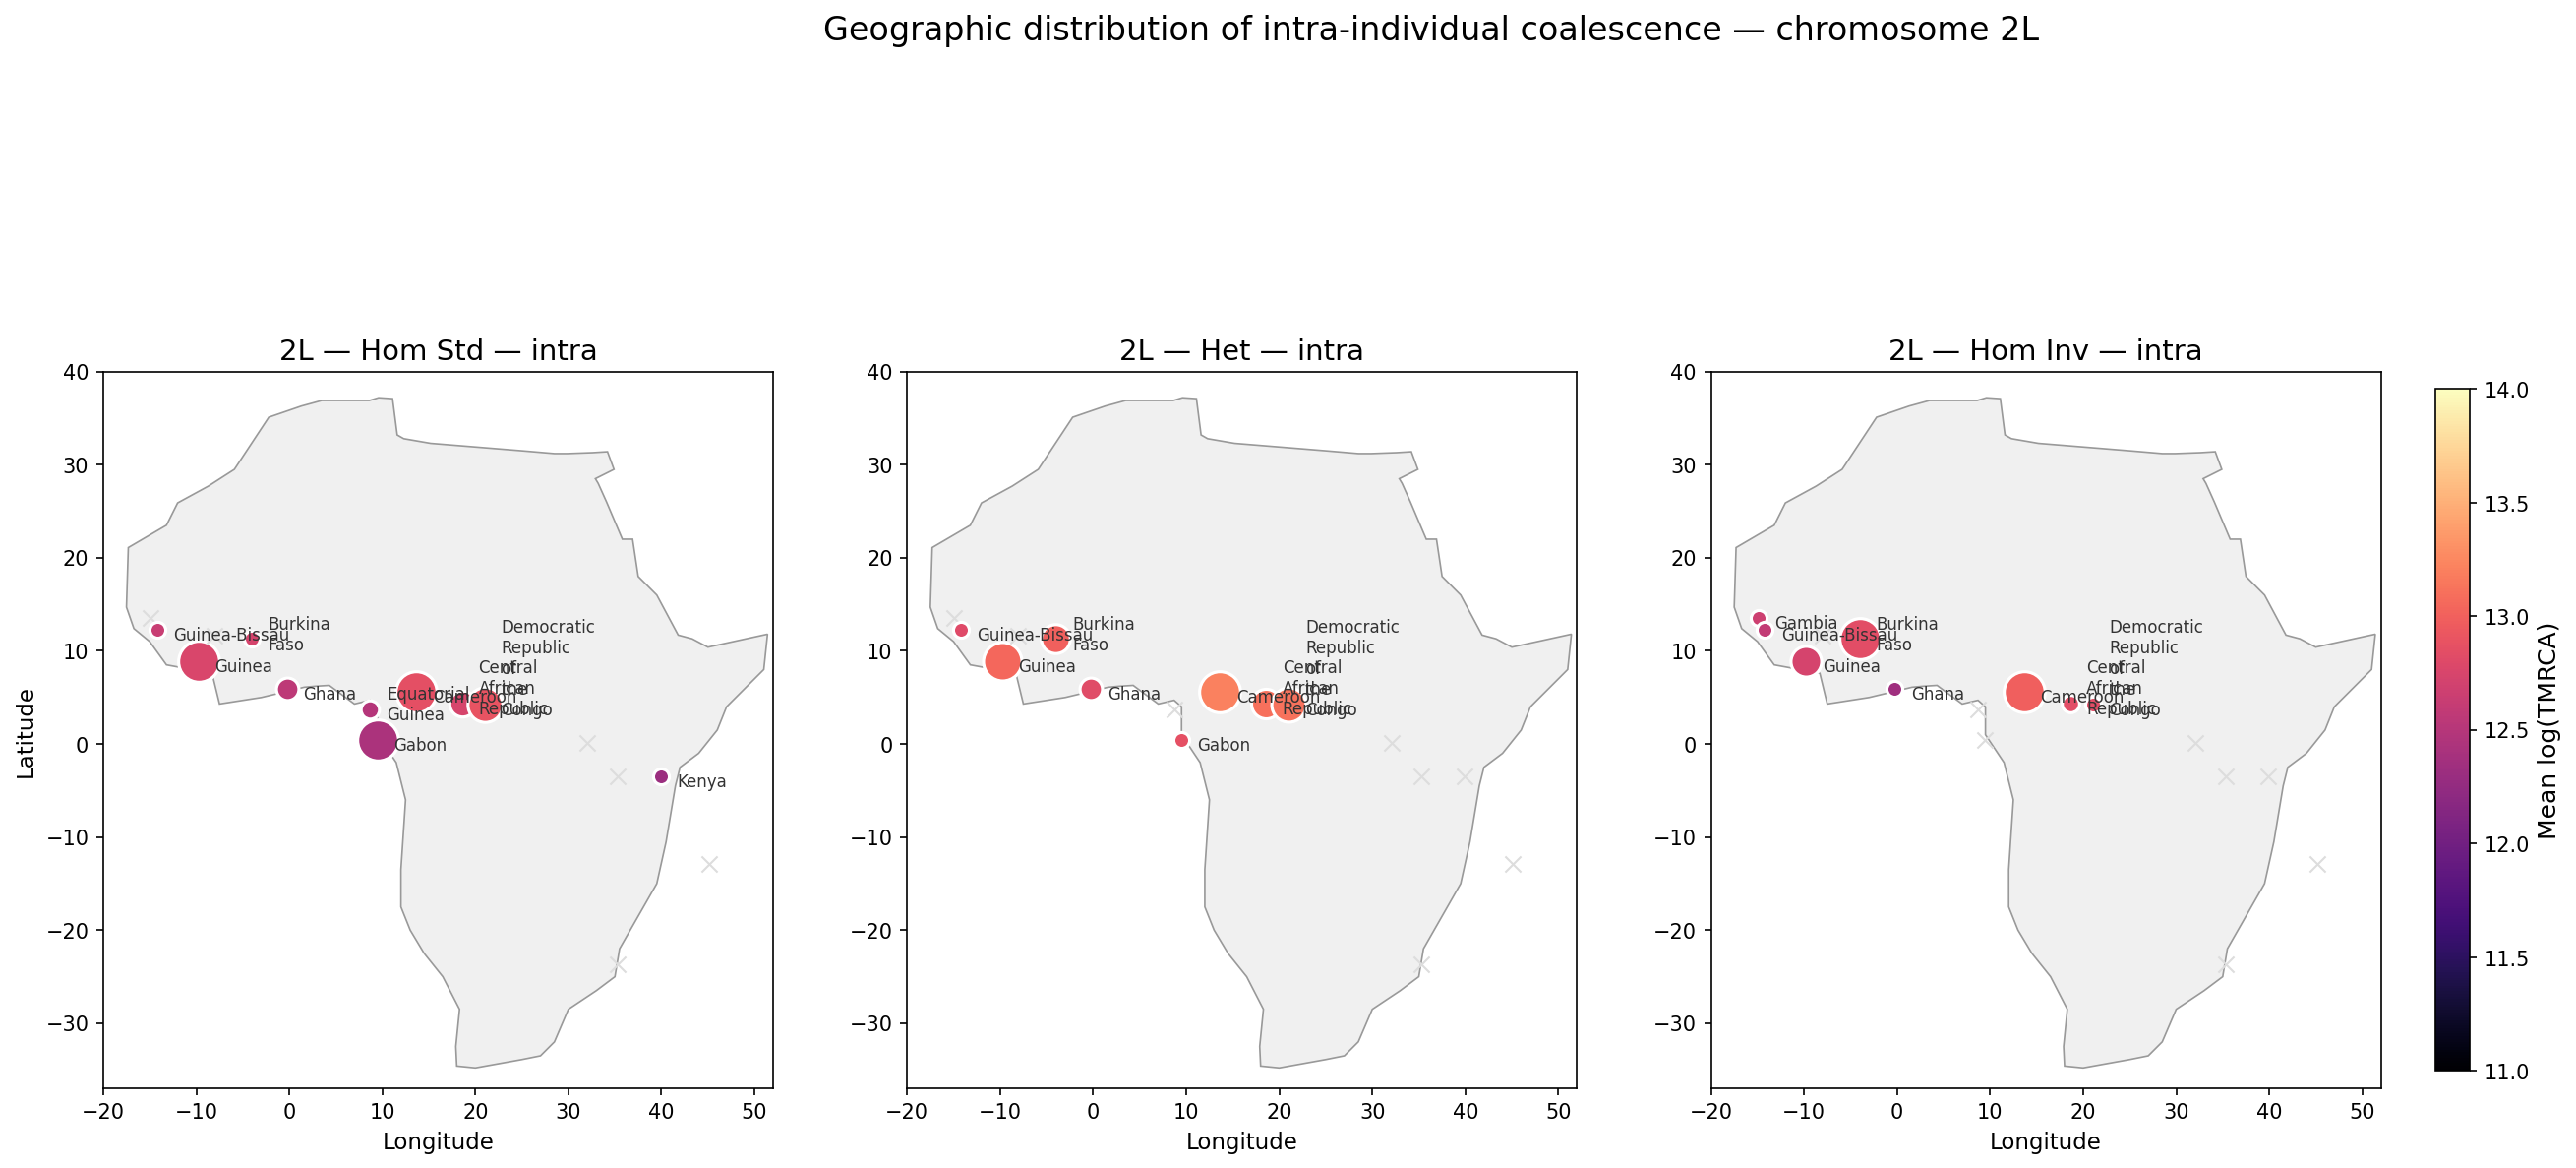
\includegraphics[width=0.48\textwidth]{geographic/map_2L_bubbles.png}
\caption{\textbf{Population structure and geographic variation.}
\textbf{a,} Cross-population heatmap of mean log(TMRCA) across chromosome
arms, karyotype groups, and pair types.
\textbf{b,} TMRCA profiles embedded as sparklines at each population's
geographic location.
\textbf{c,} Bubble map: circle size = sample count, color = mean TMRCA.
}
\label{fig:geography}
\end{figure}

\begin{figure}[p]
\centering
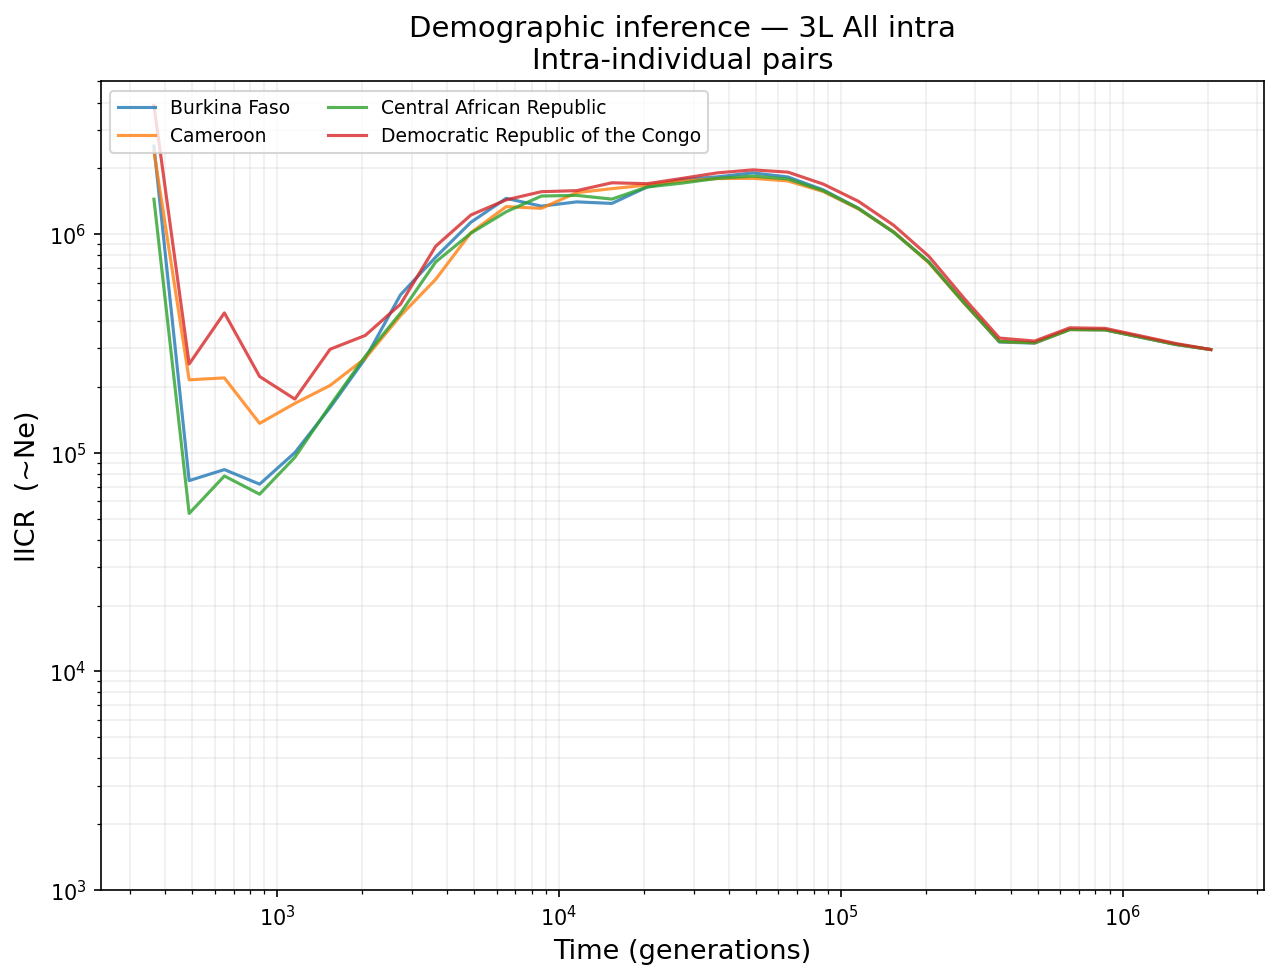
\includegraphics[width=0.85\textwidth]{demography/demography_3L_all_allpops.png}
\\[0.5em]
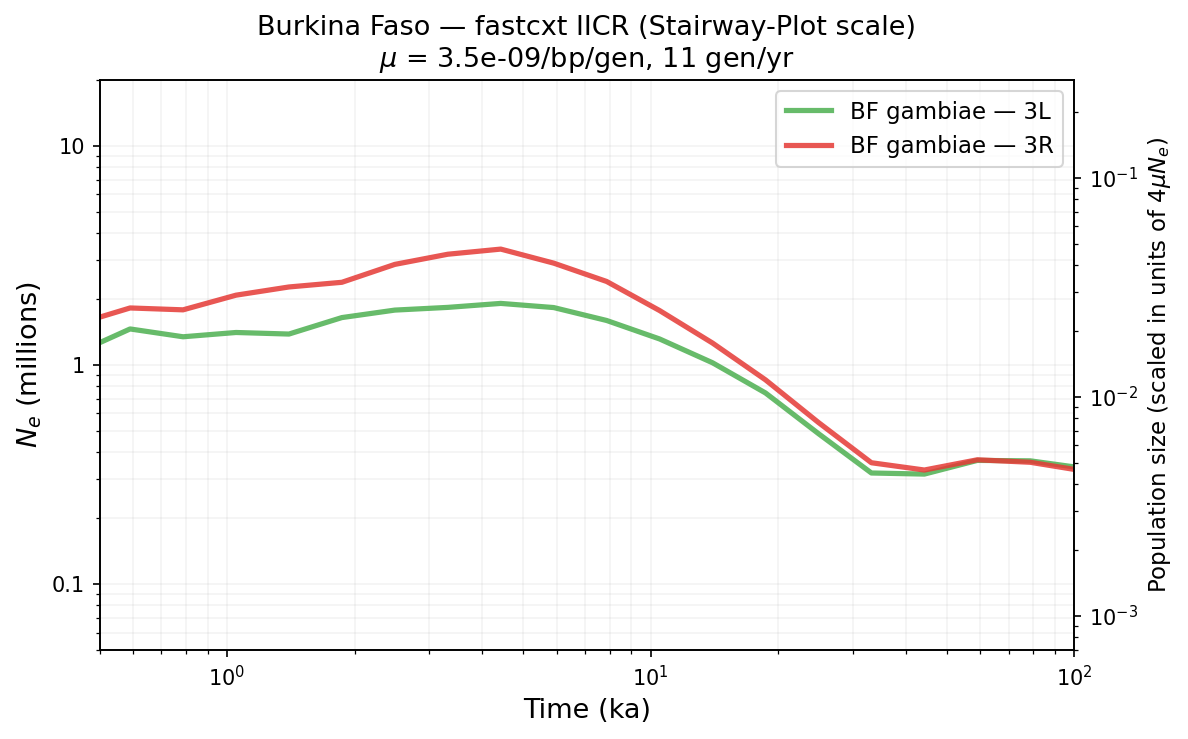
\includegraphics[width=0.45\textwidth]{demography/stairway_style_burkina_faso.png}
\hfill

\includegraphics[width=0.45\textwidth]{demography/demography_allarms_Burkina_Faso.png}
\caption{\textbf{Demographic history from coalescence time distributions.}
\textbf{a,} IICR ($\sim N_e(t)$) curves for all completed populations on
chromosome 3L (no inversions). Dashed line = stdpopsim reference model.
\textbf{b,} Stairway-plot-style demographic estimate for Burkina Faso (3L,
3R) compared with SMC++ and the reference model.
\textbf{c,} All chromosome arms overlaid for Burkina Faso. 3L and 3R
(no inversions) track the reference model; the X~chromosome shows the
expected $\sim$3/4 reduction in $N_e$.
}
\label{fig:demography}
\end{figure}

% ======================================================================
% ONLINE METHODS
% ======================================================================

\clearpage
\section*{Methods}

\subsection*{Data}

We used phased whole-genome sequences from the Ag1000G Ag3.0
release~\citep{ag1000g2020genome}, comprising $\sim$1{,}470
\textit{An.~gambiae} individuals from 16 African populations. Ancestral
allele polarization used \textit{An.~arabiensis} as outgroup. Tree sequences
were inferred using tsinfer~\citep{kelleher2019inferring} and dated with
tsdate~\citep{wohns2022unified} for validation. Data accessibility masks
from the Ag1000G release were used to filter low-quality regions.

\subsection*{Karyotype stratification}

On chromosome arms 2L and 2R, individuals were classified as homozygous
standard, heterozygous, or homozygous inverted for In(2L)\textit{a} and
In(2R)\textit{b} respectively, using karyotype calls from the Ag1000G
metadata. Arms 3L, 3R, and X were treated as a single group per population.

\subsection*{Model architecture}

fastcxt uses a bidirectional Mamba-2 state-space model~\citep{gu2023mamba,
dao2024transformers} as the core sequence encoder. Input genotype data are
represented as a two-channel site frequency spectrum (SFS) computed from XOR
and XNOR channels across haplotype pairs~\citep{korfmann2025cxt}. A
multi-scale convolutional stem with parallel 1D convolutions (kernel sizes 3,
11, 31, 63) captures spatial patterns at multiple resolutions. The mutation
rate is injected via Feature-wise Linear Modulation
(FiLM)~\citep{perez2018film}, providing learned scale and shift parameters at
the first and last encoder layers.

The architecture comprises a 6-layer bidirectional Mamba encoder and a
4-layer decoder with U-Net-style skip connections. Each BiMamba block runs the
state-space model in both forward and backward directions, merging
bidirectional states through a learned projection. The output head predicts
both the mean and log-variance of log(TMRCA) at each genomic window, trained
with Beta-NLL loss ($\beta = 0.5$) for calibrated heteroscedastic
uncertainty~\citep{seitzer2022pitfalls}.

\subsection*{Training}

Models were trained on simulated data generated with msprime~\citep{kelleher2016efficient}
using the \textit{An.~gambiae} Gabon demographic model from
stdpopsim~\citep{stdpopsim2020catalog}. Training used 200 simulated tree
sequences per configuration, with AdamW optimization, cosine learning rate
schedule (max LR = $3 \times 10^{-4}$), and bfloat16 mixed precision.
Cross-species validation confirmed that the architecture generalizes without
modification between human-like and mosquito training scenarios.

\subsection*{Node-time model and scaling}

To overcome the $O(n^2)$ cost of pairwise inference, we introduce a node-time
model that predicts all $n-1$ internal node times in a tree from topology
features (node rank, subtree sizes) in a single forward pass. Pairwise TMRCA
for any pair is then recovered via $O(1)$ lowest common ancestor (LCA) lookup
on the tree, achieving overall $O(n)$ scaling. For $n = 30$--$100$ samples,
this provides 7--11$\times$ speedup over the pairwise baseline
(Supplementary Table~S3).

\subsection*{Inference protocol}

Genomes were tiled into 100\,kb blocks, each yielding 500 windows of
200\,bp. For each population, karyotype group, and chromosome arm, all
within-individual (intra) haplotype pairs were processed in batches of 64
on a single GPU. Per-pair diversity-based bias correction aligned genome-wide
mean coalescence to account for demographic mismatch between training and
target populations. Results were assembled into a TimeAtlas data structure
supporting efficient queries by pair, window, or genomic region.

\subsection*{Outlier detection}

For each population, arm, and karyotype group, we computed per-block mean
log(TMRCA) and identified blocks in the 5th or 95th percentile of the
genome-wide distribution. Edge trimming (variable per arm) removed blocks
near telomeres and centromeres where data quality is reduced. Blocks were
further classified as ``credible'' (accessibility fraction $\geq 80\%$) or
``suspect'' (low accessibility). Gene annotations from VectorBase AgamP4
were overlaid using adjustText for non-overlapping label placement.

\subsection*{Demographic inference}

The inverse instantaneous coalescence rate (IICR) was computed from the
empirical TMRCA distribution as a non-parametric proxy for $N_e(t)$.
Coalescence times were binned into 200 intervals, and the rate was estimated
as the number of coalescence events per surviving pair per unit time.
Comparison with SMC++~\citep{terhorst2017robust} used the Burkina Faso
population on chromosome 3L with the first 20 samples.

% ======================================================================
% DATA AND CODE AVAILABILITY
% ======================================================================

\subsection*{Data availability}

Ag1000G data are available from the MalariaGEN resource centre.
Genome-wide coalescence time maps (TimeAtlas format) for all 16 populations
will be deposited at a public repository upon publication. Simulated training
data are reproducible via stdpopsim commands provided in the Supplementary
Methods.

\subsection*{Code availability}

fastcxt is available at \url{https://github.com/kevinkorfmann/fastcxt}
under an open-source license. Analysis scripts for reproducing all figures
are in the \texttt{experiment\_burkina\_faso/figures/} directory.

% ======================================================================
% REFERENCES
% ======================================================================

\bibliographystyle{plainnat}
\bibliography{references}

\end{document}
